\documentclass[11pt]{article}
\usepackage[a4paper,margin=25mm]{geometry}
\usepackage{amsmath,amssymb,amsthm,mathtools,booktabs,graphicx}
\usepackage[hidelinks]{hyperref}
\newtheorem{theorem}{Theorem}[section]
\newtheorem{lemma}[theorem]{Lemma}
\newtheorem{proposition}[theorem]{Proposition}
\newtheorem{corollary}[theorem]{Corollary}
\newcommand{\E}{\mathbb E}
\newcommand{\Var}{\operatorname{Var}}
\newcommand{\KL}{\operatorname{KL}}
\newcommand{\ind}{\mathbf 1}
\setlength{\parskip}{4pt}
\setlength{\parindent}{0pt}
\setlength{\emergencystretch}{2em}
\title{Rare-event threshold estimation: a critical-margin upper bound,\\a stopping obstruction, and an audited research checkpoint}
\author{AI-assisted research in the adaptive-threshold-estimation repository}
\date{27 October 2026}
\begin{document}
\maketitle
\begin{abstract}
The arbitrary-law rare-event minimax conjecture remains unresolved in this
checkpoint. A new paper proof supplies an unbiased observable estimator under
a quadratic margin envelope with second moment at most $165\rho/56$ and
mean work at most $1350a^{-2}L(1+\log L)$, where $L=1+\log(1/\rho)$.
Its budgeted risk is within a factor of order $\sqrt{1+\log L}$ of the
audited candidate lower bound for the exact quadratic law. We neither remove
this factor nor prove it necessary. A counterexample shows that one-law finite
expected stopping time cannot transfer almost-sure termination to the other
law in an unbounded fresh-coin reservoir. A corrected finite-prefix testing
principle explains the role of uniform budgets. An elementary qualified
unknown-rarity guarantee and an arbitrary-law finite upper bracket are also
given. New direct-observation experiments have mixed and sometimes poor
performance; no practical superiority is established. Primary-source
comparison identifies the exact scope of the inherited nested-simulation
lower bound and important model exclusions. All new statistical theorems are
paper proofs, not Lean proofs; novelty and external specialist review remain
unresolved. The v4 paper and frozen baselines are preserved.
\end{abstract}

\section{Experiment, computation, and evidence contract}
A fresh opaque coin independently draws $D\sim\mu$ on $(0,1/2]$ and
$S\mid D=d\sim\operatorname{Bernoulli}(q(d))$. Its retained probability is
$P=1/2+(2S-1)D$. Observations of that coin are conditionally iid Bernoulli($P$).
The algorithm observes only bits and identities. It may create, revisit,
interleave, abandon, and stop. Every requested observation costs one;
independent randomization and finite deterministic computation are uncharged.
Creating unused coins gives no information and can be deferred to first use.
No magnitude-selected query, sign oracle, or oracle for $q$ is supplied.

For known $0<\rho\le1/4$, define
\[
 \mathcal Q_\rho(\mu)=\{q\text{ measurable}:0\le q\le1,
                 \ \int q\,d\mu\le\rho\},\qquad \theta=\int q\,d\mu.
\]
This is a global constraint; $q(d)$ may equal one on a small region.
$R_{\mu,\rho}(B)$ is the infimum of worst-case RMS error over algorithms with
$\sup_{q\in\mathcal Q_\rho}\E_qT\le B$.
$r_{\mu,\rho}(B,\delta)$ is the infimum radius for which an algorithm under
the same uniform expected-work constraint has
$\sup_q\Pr_q(|\widehat\theta-\theta|>r)\le\delta$.
Algorithms and their design constants may depend on known $\mu,\rho,B,\delta$.
The new critical-envelope algorithm uses only $a,\rho,B,\delta$, not $\mu$.

For arbitrary known laws, the finite upper bracket below permits precomputed
real integral constants or certified upper bounds. This is the mathematical
known-law minimax convention, not a universal computability theorem for every
representation of a measure. A sampled coin's magnitude remains hidden.
Infinite arithmetic operations between two observations are not allowed.
An explicit experiment exists on a countable product of independent magnitude
variables, uniform variables producing signs, and uniform flip tapes. All
algorithms below make finite operations at each step and have the stated
termination property. Their random seed is independent of this product.

\paragraph{Pinned baseline.}
Initial HEAD was \texttt{ddf950122776a059e62c808021bbd2b59c39f0b0}, with
preexisting uncommitted route-a research and documentation.
The new local branch is \path{research/rare-minimax-20261027}.
Concurrent activity later
committed that inherited work and edited separate Tier 5 files; source hashes
and the precise audit scope are recorded in \path{STATE.md} and
\path{FORMAL_COVERAGE.md}. No concurrent work is credited as this run's
construction. No remote publication or researcher contact was performed.

\paragraph{Evidence labels.}
FORMALIZED means only an exact checked Lean declaration with its assumptions
and audited dependency closure. PROVED-ON-PAPER means the argument is written,
with explicit dependencies; agent review is not external peer review.
CONJECTURE, NUMERICAL, DISPROVED, and PRIOR-ART / UNRESOLVED-PRIORITY are
used literally. Exact rational finite checks certify those calculations only.
The new results below have no corresponding complete Lean statistical theorem.

\section{The candidate, inherited results, and what remains open}
The proposed functional is
\[
 \Psi_{\mu,\rho}(h)=\sup_{0\le w\le1,\,\E_\mu w\le\rho}
       \E_\mu\min\{w(D),h\sqrt{w(D)}/D\}.
\]
The existing arbitrary-law optimizer is
$w_*(d)=\min\{1,t^2/d^2\}$, where $\E\min(1,t^2/D^2)=\rho$.
This variational statement is FORMALIZED in
\texttt{ThresholdHC.Tier3.arbitrary\_law\_optimizer}; it does not supply a
statistical algorithm. The cutoff exists uniquely for $0<\rho<1$:
dominated convergence gives continuity from zero to one, and strict increase
holds before saturation because there is positive mass above the smaller
cutoff. Atoms require no allocation of selected magnitudes.
For $h<t$ the value is
\[
 \mu(D\le h)+h\E[D^{-1}\ind_{\{h<D\le t\}}]
       +ht\E[D^{-2}\ind_{\{D>t\}}],
\]
and for $h\ge t$ it is $\rho$. The pieces agree at boundary atoms.
For a fixed gap this is $\min\{\rho,h\sqrt\rho/d\}$.
For rarity bounded below, $\rho\omega_\mu(h)\le\Psi(h)\le\omega_\mu(h)$,
by choosing $w\equiv\rho$ and by $w\le1$ respectively.
These comparisons have constants depending on the lower bound for $\rho$.

The inherited lower bound $R\gtrsim\Psi(B^{-1/2})$ (and its confidence
analogue) is PROVED-ON-PAPER with the imported Lee--Valiant Corollary 19
and a bounded-likelihood-ratio decomposition as dependencies. The source
requires simultaneous universal smallness of its prior, increment, gap,
and relative increment; it is an expected-work, history-averaged statement.
The continuation handles larger gaps separately by sign revelation and data
processing. The fresh-reservoir reduction and its limits remain paper-level.
The audit found no blocking gap in this argument; it is not an independently
formalized minimax theorem. See \texttt{REVIEW\_MATH.md} and
\texttt{LITERATURE\_AUDIT.md} for the exact inspected material.

Matching paper rates for $0<\alpha<2$ and the separate $\alpha>2$ result
were inherited, not proved for the first time by this run. For $\alpha>2$,
constants depend on $\alpha$ and diverge near two. The next section addresses
the missing critical case but leaves an iterated logarithm.
The heuristic $\rho\omega_\mu((\rho B)^{-1/2})$ remains DISPROVED:
$\mu=\rho\delta_{\rho^2}+(1-\rho)\delta_{1/4}$ and $B=\rho^{-4}$ give
true lower order $\rho$ versus heuristic order $\rho^2$.
No counterexample to $\Psi$ itself was established here.

\section{A critical-margin upper bound with a remaining iterated logarithm}
\label{sec:critical}
\noindent\textbf{PROVED-ON-PAPER.} The result below is new work in this run,
reviewed by a separate adversarial agent. It is not Lean-checked or externally
reviewed; priority is unresolved. It does not settle the candidate minimax law.
Natural logarithms are used throughout.

Assume the iid hidden-gap Bernoulli experiment of the question. Only requested
coin observations are charged; arithmetic and independent randomness are free.
For known $0<a\le1/2$, assume
\begin{equation}\label{crit:envelope}
 \mu((0,x])\le(x/a)^2\quad(0<x<a).
\end{equation}
The individual gaps, signs, and unknown measurable function $q$ remain hidden.
Only the global condition $\int q\,d\mu\le\rho$ is imposed, with known
$0<\rho\le1/4$. Set $L=1+\log(1/\rho)$ and $H=1+\log L$.

\begin{theorem}\label{crit:theorem}
There is an observable single-coin estimator $Y$, depending only on $a,\rho$,
such that uniformly over \eqref{crit:envelope} and every admissible $q$,
\[
 \mathbb EY=\theta,\qquad
 \mathbb EY^2\le\frac{165}{56}\rho<4\rho,\qquad
 \mathbb ET_Y\le W:=1350a^{-2}LH.
\]
Thus, for every $B>0$, an algorithm of uniform expected work at most $B$ has
worst-case RMS at most
\[
 \min\left\{\rho/2,\sqrt{5400\rho LH/(a^2B)}\right\}.
\]
For $0<\delta\le1/4$, let $k$ be the least odd integer at least
$8\log(1/\delta)$. A confidence radius
\[
 \min\{\rho/2,4\sqrt{\rho Wk/B}\}
\]
is attainable with the same uniform expected-work budget. These statements
give no deterministic work cap or high-probability work bound.
\end{theorem}

\subsection{An entirely observable finite classifier}
For $j\ge0$, put
\[
 \varepsilon_j=16^{-(j+1)},\quad
 N_j=\left\lceil(a^2\rho\varepsilon_j)^{-1}\right\rceil,\quad
 K_j=\left\lceil\log_2(a\sqrt{N_j})\right\rceil.
\]
For $0\le k\le K_j$, let $r_k=a2^{-(k+1)}$. If $H_n$ is the number of
observed heads after $n$ flips of the current coin, define
\[
 L^+_{k,n}=(1+2r_k)^{H_n}(1-2r_k)^{n-H_n},\qquad
 L^-_{k,n}=(1-2r_k)^{H_n}(1+2r_k)^{n-H_n}.
\]
At each $n<N_j$, output zero and stop if some $L^-_{k,n}$ reaches
$(K_j+1)/\varepsilon_j$, or output one and stop if some $L^+_{k,n}$ reaches
$(K_j+1)/(\rho\varepsilon_j)$. Give zero priority in a simultaneous crossing.
If neither decision has occurred before $N_j$, output
$\mathbf1_{\{H_{N_j}>N_j/2\}}$. Call the output $Z_j$ and work $T_j$.
Only finitely many likelihoods are checked at any time.

Under the wrong sign the corresponding likelihood is a nonnegative
supermartingale with expected multiplier $1-4r_kd\le1$. Applying the
bounded-horizon crossing inequality to each of the $K_j+1$ likelihoods gives
wrong-crossing probability at most $\varepsilon_j$ on positives and
$\rho\varepsilon_j$ on negatives. The wrong forced-majority event is a
subset of the full-tape majority-error event, whose conditional probability
is at most $\exp(-2N_jd^2)$ by Hoeffding. No independence between stopping
and this event is used. Stochastic dominance from \eqref{crit:envelope} yields
\[
 \mathbb E_\mu e^{-2ND^2}
 \le\frac{1-e^{-2Na^2}}{2Na^2}\le\frac1{2Na^2}.
\]
Consequently, for every admissible $q$,
\begin{equation}\label{crit:error}
 \mathbb P(Z_j\ne S)\le\tfrac52\rho\varepsilon_j,
 \qquad
 \mathbb P(Z_j=1,S=0)\le\tfrac32\rho\varepsilon_j.
\end{equation}
The $\theta\varepsilon_j$ positive error was bounded by
$\rho\varepsilon_j$; the assumption was never strengthened to $q(d)\le\rho$.
For completeness, the concentration input has a direct Bernoulli proof:
the centered log moment-generating function $\phi(\lambda)$ has
$\phi(0)=\phi'(0)=0$ and $\phi''(\lambda)\le1/4$, because the tilted
Bernoulli variance is at most $1/4$. Hence $\phi(\lambda)\le\lambda^2/8$.
Multiply these bounds for independent observations and apply Markov's
inequality with $\lambda=4d$ (or $-4d$) to obtain $e^{-2Nd^2}$.
This argument also applies to the independent failure indicators used below.

\subsection{Conditional work and global-rarity rearrangement}
Write $x=\min(d,a)$ and
\[
 A_s=1+\log(K_j+1)+\log(1/\varepsilon_j)+s\log(1/\rho),\quad s=0,1.
\]
If $x\ge N_j^{-1/2}$, choose $k=\lceil\log_2(a/x)\rceil\le K_j$.
Then $x/4\le r_k\le x/2$, $r_k\le1/4$, and the correct-sign log-likelihood
has iid increments with mean
\[
 g=\tfrac12\log(1-4r_k^2)
       +d\log\frac{1+2r_k}{1-2r_k}
 \ge-\tfrac83r_k^2+4dr_k\ge\tfrac23x^2.
\]
Here $\log(1-z)\ge-z/(1-z)$ and
$\log((1+u)/(1-u))\ge2u$ suffice. Every upward increment is less than one.
For the crossing time $\sigma$ of the correct threshold, the bounded
stopped-sum identity at $\sigma\wedge n$ gives
$g\mathbb E(\sigma\wedge n)\le A_s$. Monotone convergence therefore gives
$\mathbb E\sigma\le(3/2)A_s/x^2$. The capped classifier work is at most
$\min(N_j,\sigma)$, including when the crossing occurs exactly at the cap.
If $x<N_j^{-1/2}$ the same conclusion below holds trivially because $A_s\ge1$:
\begin{equation}\label{crit:condwork}
 \mathbb E(T_j\mid d,s)\le\min\{N_j,(3/2)A_s/x^2\}.
\end{equation}

Set $c=3/2$. For the negative-sign contribution stochastic dominance gives
\[
 \mathbb E\min\{N,cA_0/x^2\}
 \le cA_0a^{-2}[1+\log_+(Na^2)].
\]
For positives, layer cake and
$\mathbb E[q\mathbf1_E]\le\min\{\rho,\mu(E)\}$ give
\begin{align*}
 \mathbb E\bigl[q(D)\min\{N,cA_1/x^2\}\bigr]
 &\le cA_1a^{-2}[1+\log_+(Na^2\rho/(cA_1))]\\
 &\le cA_1a^{-2}[1+\log_+(Na^2\rho)].
\end{align*}
Indeed the sharp upper is the integral of
$\min\{N,cA_1/(a^2u)\}$ over $0<u<\rho$. If
$Na^2\rho\le cA_1$ this is $N\rho\le cA_1/a^2$; otherwise it is exactly
$(cA_1/a^2)[1+\log(Na^2\rho/(cA_1))]$. This proof also covers envelope laws
with atoms, through layer cake rather than a quantile-density assumption.
Bounding the negative part by the full unweighted integral and adding the
positive part bounds $\mathbb ET_j$.

The following loose universal bounds follow directly from the definitions:
\[
 \begin{gathered}
 N_ja^2\le2/(\rho\varepsilon_j),\qquad K_j+1\le5(L+j+1),\\
 A_0\le7H(j+1),\qquad A_1\le7H(j+1)+L,\\
 1+\log(N_ja^2)\le5L(j+1),\qquad
 1+\log(N_ja^2\rho)\le5(j+1).
 \end{gathered}
\]
For example, use $\log(L+j+1)\le\log L+j+1$ and $4\log2<3$ in the
bound on $A_0$. Since $L,H\ge1$, substitution proves
\begin{equation}\label{crit:work}
 \mathbb ET_j\le(225/2)a^{-2}LH(j+1)^2.
\end{equation}

\subsection{Randomized telescoping and exact expected-budget aggregation}
Independently draw $J$ with $p_j=2^{-(j+1)}$, then draw a fresh coin. For
$J=0$, set $\Delta_0=Z_0$. For $J=j\ge1$, run $Z_j$ and $Z_{j-1}$ on
two successive disjoint observation blocks of that \emph{same} coin and set
$\Delta_j=Z_j-Z_{j-1}$. Return $Y=\Delta_J/p_J$.

Conditional on $(D,S)$, the observations after the first bounded stopping
time again form an iid Bernoulli tape with the original parameter. To verify
this directly, condition on each possible first stopping time $n$ and each
observed length-$n$ prefix. Its event is prefix-measurable and the unused iid
coordinates have their original law. Summing the finitely many prefix events
proves the suffix assertion. Thus the second block has exactly the classifier
marginal used below; its work can be added in expectation. The two outputs
share their latent sign, which is essential to the disagreement bound.

By \eqref{crit:error},
\[
 \mathbb E\Delta_0^2\le\tfrac{35}{32}\rho,\qquad
 \mathbb E\Delta_j^2\le\tfrac{85}{32}\rho16^{-j}\quad(j\ge1).
\]
For the latter, different decisions imply that at least one is wrong about
the shared sign. Hence Tonelli gives
\[
 \mathbb EY^2\le\frac{35}{16}\rho+
      \frac{85}{16}\rho\sum_{j\ge1}8^{-j}
   =\frac{165}{56}\rho<4\rho.
\]
The same bounds give $\sum_j\mathbb E|\Delta_j|<\infty$; signed
expectations may therefore be interchanged and telescoped, giving
$\mathbb EY=\lim_j\mathbb EZ_j=\theta$. This proves integrability before
using the signed telescope. The expected work of level $j$ is at most twice
\eqref{crit:work}, and
$\sum_jp_j(j+1)^2=6$. Thus $\mathbb ET_Y\le1350a^{-2}LH$.
Every call terminates almost surely, and the resulting expected work is finite.

For budget $B$, set $\lambda=B/W$, independently draw
$M\sim\operatorname{Poisson}(\lambda)$, and average the independent fresh-coin
outputs as $\lambda^{-1}\sum_{i=1}^M Y_i$. Conditioning on $M$ proves
expectation $\theta$, variance $\mathbb EY^2/\lambda\le4\rho W/B$, and
expected work at most $B$. This remains valid for $\lambda<1$. Project onto
$[0,\rho]$, which improves squared error without preserving unbiasedness.
If the stated RMS bound exceeds $\rho/2$, choose the zero-work constant
$\rho/2$ instead. This proves the RMS assertion.

For confidence, run $k$ independent copies with budgets $B/k$ and take their
median. Each has failure probability at most $1/4$ at radius
$4\sqrt{\rho Wk/B}$ by Chebyshev. Hoeffding's inequality for the independent
failure indicators bounds median failure by $e^{-k/8}\le\delta$. If
$\rho/2$ is the smaller displayed radius, explicitly choose the constant
estimator instead. Total expected work is at most $B$.

\subsection{Exact critical candidate and the unresolved gap}
For the exact law $F(d)=(d/a)^2$, direct integration yields
\[
 \rho=(t/a)^2[1+2\log(a/t)],\qquad
 \Psi(h)=\begin{cases}
 [2ht(1+\log(a/t))-h^2]/a^2,&0<h<t,\\
 \rho,&h\ge t.
 \end{cases}
\]
Set $u=1+2\log(a/t)$. Then $\rho=u e^{1-u}$ and
$L=u-\log u$, whence $L\le u\le2L$. For $h<t$,
$\Psi(h)/h=(t/a^2)(u+1-h/t)$ lies between $tu/a^2$ and
$t(u+1)/a^2$. Since $tu/a^2=\sqrt{\rho u}/a$, including the transition
at $h=t$ proves
\[
 \Psi(h)\asymp\min\{\rho,h\sqrt{\rho L}/a\}
\]
with universal constants, jointly in $\rho,h,a$. Conditional on the audited
arbitrary-law lower theorem, Theorem~\ref{crit:theorem} therefore leaves a
factor at most $\sqrt{1+\log L}$. It improves the critical upper bracket but
does not remove this factor, prove it necessary, or establish arbitrary-law
optimality. At fixed positive $\rho$, the construction gives $B^{-1/2}$ RMS;
this fixed-rarity statement must not be confused with a uniform rare-event
matching theorem.

\section{A finite, arbitrary-law upper bracket}
\noindent\textbf{PROVED-ON-PAPER; established allocation principle.}
The classifier analysis also gives a constructive upper bracket for every
law on $(0,1/2]$, including atoms, singular laws, and infinite inverse moments.
No comparison of this bracket to $\Psi$ is asserted.

Set $a=1/2$. Choose finitely many integer caps $N_j\ge4$ and tolerances
$0<\varepsilon_j\le1$, $0\le j\le m$, and use the preceding classifiers.
Let
\[
 \beta_j=\mathbb E_\mu e^{-2N_jD^2},\quad
 e_j=2\rho\varepsilon_j+\beta_j,\quad
 A_{j,s}=1+\log(K_j+1)+\log(1/\varepsilon_j)+s\log(1/\rho).
\]
For a bounded nonnegative measurable function $f$, define
\[
 Q_\rho(f)=\int_0^\infty\min\{\rho,\mu(f>v)\}\,dv.
\]
Layer cake gives $\int qf\,d\mu\le Q_\rho(f)$ for every feasible $q$.
Equality follows by choosing the largest $\rho$ mass of $f$, with a fractional
value of $q$ on a cutoff atom. Thus this formula does not require a nonatomic
law. Put
\[
 f_{j,s}(d)=\min\{N_j,(3/2)A_{j,s}/d^2\},\qquad
 c_j=\mathbb E f_{j,0}+Q_\rho(f_{j,1}).
\]
The preceding conditional-work proof gives a uniform bound $c_j$; all these
integrals are finite because the functions are bounded. Let
\[
 v_0=\rho+\rho\varepsilon_0+\beta_0,\quad C_0=c_0,
 \qquad v_j=e_j+e_{j-1},\quad C_j=c_j+c_{j-1}\quad(j\ge1).
\]
Use independent copies of the same-coin increments, independently across
levels. With $S_m=\sum_{j=0}^m\sqrt{v_jC_j}$, independently take
Poisson numbers of copies at means
$\lambda_j=B\sqrt{v_j/C_j}/S_m$. Their sum, with level $j$ divided by
$\lambda_j$, has expectation $\mathbb EZ_m$, variance at most $S_m^2/B$,
and expected work at most $B$. Therefore
\[
 R_{\mu,\rho}(B)\le
 \min\{\rho/2,\sqrt{e_m^2+S_m^2/B}\}.
\]
All constants here are positive. The RMS bound uses the exact bias--variance
identity, and clipping onto $[0,\rho]$ cannot increase risk.

The known law can determine these finitely many design constants, or certified
upper bounds on them, before sampling. This gives no access to the magnitude
of a sampled coin. For an abstract probability measure this is existence at
the fixed known law; uniform computability from every representation of a
measure is not claimed. Floating-point quadrature alone supplies numerical
design evidence, not certified risk constants. The Poisson allocation and
randomized telescoping principles are established methods; no novelty is
claimed for them.

\section{A reusable bounded-channel upper principle}
\noindent\textbf{PROVED-ON-PAPER; no lower transfer.}
The critical theorem and arbitrary-law upper bracket hold with the same
constants if each hidden state produces conditionally iid observations
$X\in[0,1]$ of mean $1/2+(2S-1)D$. Charge one unit per observation; the
algorithm receives no hidden magnitude, sign, or selected-state access.
Replace the reference processes by
\[
 M^\pm_{k,n}=\prod_{i=1}^n[1\pm2r_k(2X_i-1)]
\]
and keep the same thresholds, caps, and empirical-mean decision. The factors
are positive. Under the wrong sign their conditional mean is $1-4r_kd\le1$.
For the correct sign, concavity of the logarithm gives
\[
 \log(1+2r(2X-1))\ge
 X\log(1+2r)+(1-X)\log(1-2r).
\]
Its expected log increment is therefore at least the Bernoulli drift used
above; upward increments remain below one. For the concentration step the
second derivative of a centered log moment-generating function is the variance
under a tilted law on $[0,1]$, at most $1/4$. Hence the previous mgf proof
applies. All conditional work, global-rarity integration, and telescoping
arguments carry over unchanged. This rule directly uses the real observations.

For a concrete derived synthetic example, take, conditional on $d,s$,
\[
 X\sim\operatorname{Unif}
 [1/2+(2s-1)d-1/4,\;1/2+(2s-1)d+1/4],
 \quad 0<d\le a\le1/4.
\]
With independent noises on revisits this is a valid bounded channel with
variance $1/48$. The quadratic-margin upper theorem applies, charging one
real draw per step. No minimax equality or empirical application is asserted.

An exact information-discarding reduction is also available: using an
independent $U\sim\operatorname{Unif}[0,1]$, the variable
$\mathbf1_{\{U\le X\}}$ is a Bernoulli observation with the required
conditional mean. One real observation is charged per converted bit and the
target is unchanged. This transfers Bernoulli upper algorithms; it does not
transfer a Bernoulli lower bound to every channel. If instead $X$ is
deterministically its conditional mean, one observation reveals $S$, and $n$
fresh states yield variance at most $\rho/n$ without an inverse-gap factor.
Nothing here extends a bounded-observation theorem to unbounded observations.

Extra cross-state structure also changes the question. As an explicit
different experiment, suppose the outer state $Z\sim\operatorname{Unif}[-1,1]$
is observed, $\beta\in[-1/2,1/2]$ is unknown, and
\[
 X=\tfrac12+(Z-\beta)/8+\xi,\qquad
 \xi\sim\operatorname{Unif}[-1/16,1/16].
\]
Independent pairs have $X\in[0,1]$, and the positive-mean fraction is
$\theta=(1-\beta)/2$. The average of $Z-8(X-1/2)$ is unbiased for $\beta$
with variance $1/(12n)$; the corresponding estimate of $\theta$ has variance
$1/(48n)$. Charging one unit per outer draw and one per inner observation
gives work $2n$. The margin near zero is linear, yet this common regression
parameter permits $B^{-1/2}$ RMS without a margin logarithm. Observed states
and cross-state structure are explicit extra information, so this calculation
does not contradict the hidden unstructured reservoir lower theorem.

% Self-contained fragment for the research note; paper proof, not Lean-checked.
\section{A necessary correction to the countable-reservoir bridge}
\paragraph{Evidence status.}
The next two propositions are PROVED-ON-PAPER in this run. Their stochastic
statements are not Lean-checked. Exact rational finite-prefix checks are reported
separately and do not certify the infinite-horizon calculation. The finite-coin
Tier 3 theorem is unchanged and is not contradicted.

\begin{proposition}[One-law finite work does not transfer termination]
Consider fresh iid coins with deterministic gap $D=1/2$. Under $P$ their positive
sign probability is $5/8$, and under $Q$ it is $3/8$. Query each coin once. If
$X_i$ is its observed bit, stop at
\[
 T=\inf\{n\ge1:\ \textstyle\sum_{i=1}^n(2X_i-1)=1\}.
\]
Then $P(T<\infty)=1$, $\mathbb E_P T=4$, whereas
$Q(T<\infty)=3/5$. In particular $Q(T=\infty)=2/5$.
\end{proposition}
\begin{proof}
For iid bits of parameter $p$, put $q=1-p$. A first hit at time $2k+1$ has
$k+1$ upward and $k$ downward steps, and the first $2k$ partial sums never
exceed zero. The number of such paths is the Catalan number
$C_k=(k+1)^{-1}\binom{2k}{k}$. This follows by reflecting at the first
forbidden positive step: among paths with $k$ up and $k$ down steps, the
forbidden paths are counted by $\binom{2k}{k+1}$, whose subtraction gives
$C_k$. Thus
\[
 \Pr_p(T=2k+1)=C_kp^{k+1}q^k.
\]
The generating series $C(z)=\sum_{k\ge0}C_kz^k$ satisfies
$C(z)=1+zC(z)^2$: split a nonempty Catalan path at its first return to zero.
The solution continuous at zero with $C(0)=1$ is
$C(z)=(1-\sqrt{1-4z})/(2z)$ for $0\le z<1/4$.
Consequently the probability generating function, excluding the mass at
infinity, is
\[
 G_p(s)=\mathbb E_p[s^T;T<\infty]
       =psC(pqs^2)=\frac{1-\sqrt{1-4pqs^2}}{2qs},\qquad 0<s\le1.
\]
For $p\ne1/2$ all series converge in a neighborhood of $s=1$.
It follows that $G_p(1)=1$ when $p>1/2$, and $G_p(1)=p/q$ when $p<1/2$.
For $p>1/2$, differentiation gives $G_p'(1)=1/(2p-1)$.
Equivalently differentiate $G_p(s)=s[p+qG_p(s)^2]$ at $s=1$;
nonnegative-series differentiation computes $\mathbb E_pT$ because
$G_p(1)=1$. Substituting $p=5/8$ and $p=3/8$ gives the claims.
\end{proof}

The example lies exactly in the symmetric prior family $1/2\pm\eta$ with
$\eta=1/8$. It also has an interior-gap variant: choose $D=1/4$, retain the
same sign priors, and use only the first observation of each fresh coin.
The observed bits then have parameters $9/16$ and $7/16$; the same calculation
gives $\mathbb E_PT=8$ and $Q(T=\infty)=2/9$. Thus deterministic coin
endpoints are not responsible for the failure. For a fixed finite coin family,
the two latent-prior laws have a globally bounded likelihood ratio; for an
unbounded reservoir that finite-family comparison is unavailable.

This example still has finite full-transcript relative entropy. On every finite
stopped path the upward step count exceeds the downward count by one, so the
likelihood ratio $dP/dQ$ is $5/3$. On infinite paths it is zero, since P has no
such mass. Therefore $\operatorname{KL}(P,Q)=\log(5/3)$. It is consistent with
the proposed full-transcript bound at $h=1/2$: convexity of $1/x$ gives
$\log(5/3)\le8/15<128/225=(128/225)h^2\mathbb E_PT$.
Thus full KL can extend while the two-law stopping transfer cannot.

\begin{proposition}[Finite-prefix information implies terminal testing]
Let $P,Q$ describe a common policy with independent seed included in increasing
observable prefix sigma fields $\mathcal F_n$. Let $T$ be its stopping time.
Assume $T<\infty$ almost surely under each law and $\mathbb E_PT\le B<\infty$.
Suppose, for a constant $k\ge0$, every finite-prefix transcript satisfies
\[
 \operatorname{KL}(P|_{\mathcal F_n},Q|_{\mathcal F_n})
       \le k\mathbb E_P(T\wedge n).
\]
If a terminal test $\phi\in\{0,1\}$ has
$P(\phi=1)\ge1-\delta$ and $Q(\phi=1)\le\delta$, with $0<\delta<1/2$, then
\[
 \operatorname{kl}(1-\delta,\delta)\le kB.
\]
\end{proposition}
\begin{proof}
The event $A_n=\{T\le n,\phi=1\}$ belongs to $\mathcal F_n$ because the
test is measurable at stopping. Let $p_n=P(A_n)$ and $q_n=Q(A_n)$.
Then $p_n\ge1-\delta-P(T>n)\ge1-\delta-B/n$, while $q_n\le\delta$.
For all sufficiently large $n$, $1-\delta-B/n>\delta$.
Data processing for the binary indicator of $A_n$, and monotonicity of binary
relative entropy in its first argument above its second, and in its second
argument below its first, give
\[
 \operatorname{kl}(1-\delta-B/n,\delta)
 \le\operatorname{kl}(p_n,q_n)
 \le\operatorname{KL}(P|_{\mathcal F_n},Q|_{\mathcal F_n})\le kB.
\]
Continuity at $(1-\delta,\delta)$ proves the result by $n\to\infty$.
The case $q_n=0<p_n$ gives infinite binary relative entropy and cannot occur
under a finite information bound. No transfer of termination from $P$ to $Q$
has been used. Separate finite expected-work bounds under the two laws are
a sufficient condition for the stated two termination assumptions.
\end{proof}

\paragraph{Canonical numbering and the remaining formal obligation.}
After $n$ charged observations, at most $n$ coin identities have been observed.
Assign indices $1,\ldots,n$ in order of first observation and retain a dictionary
for revisits. Every unobserved iid latent draw can be deferred until its first
observation: prior decisions involving its label contain no information about
that draw. This recursive construction preserves the observed finite-prefix law
and the number of charged observations. It requires that each action completes
after finite computation; infinitely many cost-free operations do not constitute
an observation oracle. For the symmetric information bound, condition on the
first $n$ iid magnitudes and the independent seed, apply the deterministic-gap
finite-prefix bound, and integrate. Magnitudes may be appended for this upper
bound on information and then removed by data processing; the policy itself
does not observe them. For the rare-prior bound, the appropriate single-coin
inequality and bounded-ratio hybrid decomposition must instead be used.

This is a paper-level reservoir realization and reduction, not an existing Lean
theorem. The existing finite-family declaration cannot be instantiated with a
different coin count at each horizon and thereby produce a single already
formalized infinite-reservoir process. One must formalize its joint law and
prove consistent realization of every prefix. The terminal-testing proposition
then closes the limit once those prefix bounds and the policy's admissibility
are available. The minimax experiment's uniform expected budget gives finite
work under both alternatives, so the counterexample does not invalidate the
paper minimax lower bound.

\paragraph{Reusable scope and boundary.}
The terminal-testing bridge works for any observation channel and any positive
cost accounting once its finite-prefix KL bound has been proved. With unequal
costs, a proved bound of the form
$\operatorname{KL}_n\le c\mathbb E_P\sum_{j\le T\wedge n}a_j$
gives the corresponding testing bound by the same limiting argument, provided
stopping is established separately (a positive lower bound on $a_j$ is one
sufficient condition). There is no asserted universal Bernoulli scaling for
other channels. Cross-state information can invalidate the iid coin likelihood
factorization even though this abstract testing step still holds; a shared
unknown parameter learned at one state must be included in a different
finite-prefix information calculation.

\section{A qualified guarantee when rarity is unknown}
\paragraph{Evidence status.} PROVED-ON-PAPER in this run, not Lean-checked and
not claimed original. This elementary construction supplies a sufficient
additive floor, not a matching adaptation penalty.

\begin{proposition}[Known fixed gap, unknown rarity]
Let $\mu=\delta_d$, $0<d<1/2$, be known. For budget $B\ge1$, let $m$ be the
least positive odd integer at least $\log(2B)/(2d^2)$. If $B\ge2m$, there is
one estimator independent of $\rho$ such that, for every $0\le\theta\le1$,
\[
 \mathbb E_\theta T\le B,\qquad
 \mathbb E_\theta(\widehat\theta-\theta)^2
 \le \frac{8m\theta}{B}+\frac{4m}{B^2}.
\]
Its work actually has a deterministic cap. For $B<2m$, the constant zero
has error $\theta$. These two cases specify the algorithm without knowing
$\theta$ or a rarity bound.
\end{proposition}
\begin{proof}
Set $n=\lfloor B/m\rfloor$, and query $n$ fresh coins exactly $m$ times each.
Let $Z_i$ be their strict-majority decisions. Put
\[
 f=\Pr\{\operatorname{Bin}(m,1/2-d)>m/2\}.
\]
This number is computable from $d,m$, with no access to the hidden sign.
Oddness gives positive-sign success probability $1-f$, so
$Z_i$ are iid Bernoulli with mean $p=f+(1-2f)\theta$.
Return $(\overline Z-f)/(1-2f)$, clipped to $[0,1]$.
Hoeffding's inequality gives $f\le e^{-2md^2}\le1/(2B)\le1/4$.
The raw estimator is unbiased and has variance
\[
 \frac{p(1-p)}{n(1-2f)^2}
 \le\frac{4(\theta+f)}n
 \le\frac{8m\theta}{B}+\frac{4m}{B^2},
\]
using $n\ge B/(2m)$. Clipping reduces squared error. The cost is $nm\le B$;
termination is deterministic. This proof requires no random-budget argument.
\end{proof}

Thus for a known fixed interior gap this one estimator has, uniformly over
$\theta\le\rho$, error of order at most
$\sqrt{\rho\log(2B)/(d^2B)}+\sqrt{\log(2B)}/(dB)$ in the nontrivial regime.
The logarithmic multiplicative loss and additive floor are \emph{sufficient};
the qualitative unknown-rarity impossibility does not establish either as
necessary. No claim of an optimal adaptation rate follows.

Unlike a distribution-dependent oracle radius, this construction also provides
a genuinely computable, although not rarity-sharp, confidence interval.
For $B\ge2m$, set
\[r=\frac{\sqrt{\log(2/\delta)/(2n)}}{1-2f}\]
and intersect
$[(\overline Z-f)/(1-2f)-r,(\overline Z-f)/(1-2f)+r]$ with $[0,1]$.
The Bernoulli Hoeffding inequality gives coverage at least $1-\delta$.
For smaller budgets return $[0,1]$. Exact arithmetic is the mathematical
contract; a floating approximation to $f$ must use certified bounds or add its
numerical error to the interval. This interval was not benchmarked here.

At the deterministic endpoint $d=1/2$, one flip reveals the sign, and
$n=\lfloor B\rfloor$ flips give the ordinary binomial estimator with variance
$\theta(1-\theta)/n$. It needs no rarity input and vanishes surely at
$\theta=0$. The inherited impossibility explicitly excludes this endpoint.

\paragraph{Other adaptation questions.}
The critical-margin theorem above already handles unknown individual $\mu$
inside a supplied quadratic envelope, with known $(a,\rho)$; the inherited
$\alpha>2$ construction handles its own envelope class. Neither proves
distribution-blind attainment of $\Psi$ for arbitrary unknown $\mu$.
When both $\mu$ and $\rho$ are unknown, the inherited v4 unrestricted
distribution-blind bound still applies, with its population-dependent modulus;
it is not an observable confidence radius or a rarity-optimal guarantee.
Matching necessity for qualified adaptation remains open here.


\section{What the existing nested-simulation lower bound settles}
\paragraph{PRIOR-ART / UNRESOLVED-PRIORITY.}
The detailed audit inspected primary theorem statements and relevant proofs,
not just abstracts. The v4 observed-state construction satisfies GHA's
Assumptions 2.1 and 2.4 literally. Fixing $a_0=1/4$, its normalized gap has
density
$[2a_0(1+z^2)^{3/2}]^{-1}\le2$, and every conditional standardized
$k$th absolute moment is at most $3^{k/2}$. Both constants are independent of
accuracy and the number of cells. The fixed admissible class is the union of
all finite cell constructions with arbitrary finite sign arrays. Its hard
member may depend on accuracy. A fixed finite list of cells is not the claimed
asymptotic hard instance.

Thus the inherited lower theorem concerns an unstructured observed-state
class meeting the stated adaptive-MLMC assumptions, even with selected-state
queries. A fixed per-outer-draw cost changes its upper accounting by a constant
factor. This does not establish a lower bound for the specific known Gaussian
GHA simulator, conditional-Gaussian-only classes, smooth cross-state
regression classes, or rare-event subclasses. Broadie--Du--Moallemi's
conditional-normal premise and Gordy--Juneja's joint-density premise exclude
the literal Bernoulli hard family. Smooth nested simulation and nested kernel
quadrature have additional cross-state or outer-function regularity.

The audit also located Blum--Hu's earlier adaptive good-arm fraction problem.
Inverse-binomial calibration and randomized telescoping have explicit
predecessors in Mendo/Haldane, McLeish, Rhee--Glynn, and Vihola. The inherited
audit's assertion that Lee--Valiant used a different Hellinger normalization
was wrong: Definition 14 uses the same $1-$affinity convention. This correction
is recorded separately without altering history. No priority claim follows
from this bounded search, and specialist correspondence remains unsent.

\section{Practical evidence on a fixed, disclosed suite}
\paragraph{NUMERICAL; no superiority claim.}
All four historical direct-real versus tuned-GHA cells were resimulated with
their original seeds and 500 replications each. All 2,000 raw outputs and work
counts matched exactly. At budget 16,384 the clipped RMS values remain
0.02990 for tuned GHA and 0.03910 for the historical candidate; at 65,536 they
remain 0.02012 and 0.02185. The earlier rejection is preserved.

The new suite froze implementation hashes, seven simulators, two budgets,
128 replications per cell, metrics, seeds, and exclusion rules before running
42 cells. The candidate changes the positive sample-variance threshold of a
two-level direct-real randomized telescope by $\sqrt{1+\log(1/\rho)}$.
This is a heuristic, not an implementation of the proved likelihood-test
theorem. It is compared to its symmetric ablation and the GHA Algorithm 1
inner-sampling component in a single-level, independently calibrated driver.
The latter is explicitly an altered driver, not the original tuned full
comparator; favorable results against it do not establish superiority to GHA.
All methods receive the same original real observations, with no Bernoulli
conversion. Every pilot and production observation is charged; fresh outer
counts and alternative accounting charging them are also recorded.

The models are the published GHA simulator, a rarer version, a fixed Bernoulli
gap, two separated gap scales, near-threshold negative coins, an independently
specified uniform-mean Gaussian simulator, and deterministic endpoint coins.
Their ground truths are analytic. Synthetic models are labelled synthetic.
All probabilities are nonzero. Zero, half, and supplied-rarity-half constants
are reported; some latter constants coincide with a particular simulator's
truth, a coincidence that confers no uniform guarantee.

The candidate is rejected as a general practical improvement: results are
mixed, and the near-negative model has RMS around 0.43 even at the larger
budget while the true probability is 0.05. No matched-accuracy speedup or
break-even workload is established. New fitting and tuning costs are zero;
verification, baseline replay, and historical development costs are separately
recorded. Final clipping improves squared loss but changes bias and leaves
cost unchanged. There is no confidence procedure for this heuristic, so
coverage is marked not applicable. Bootstrap intervals are descriptive only.
\begin{figure}[htbp]
 \centering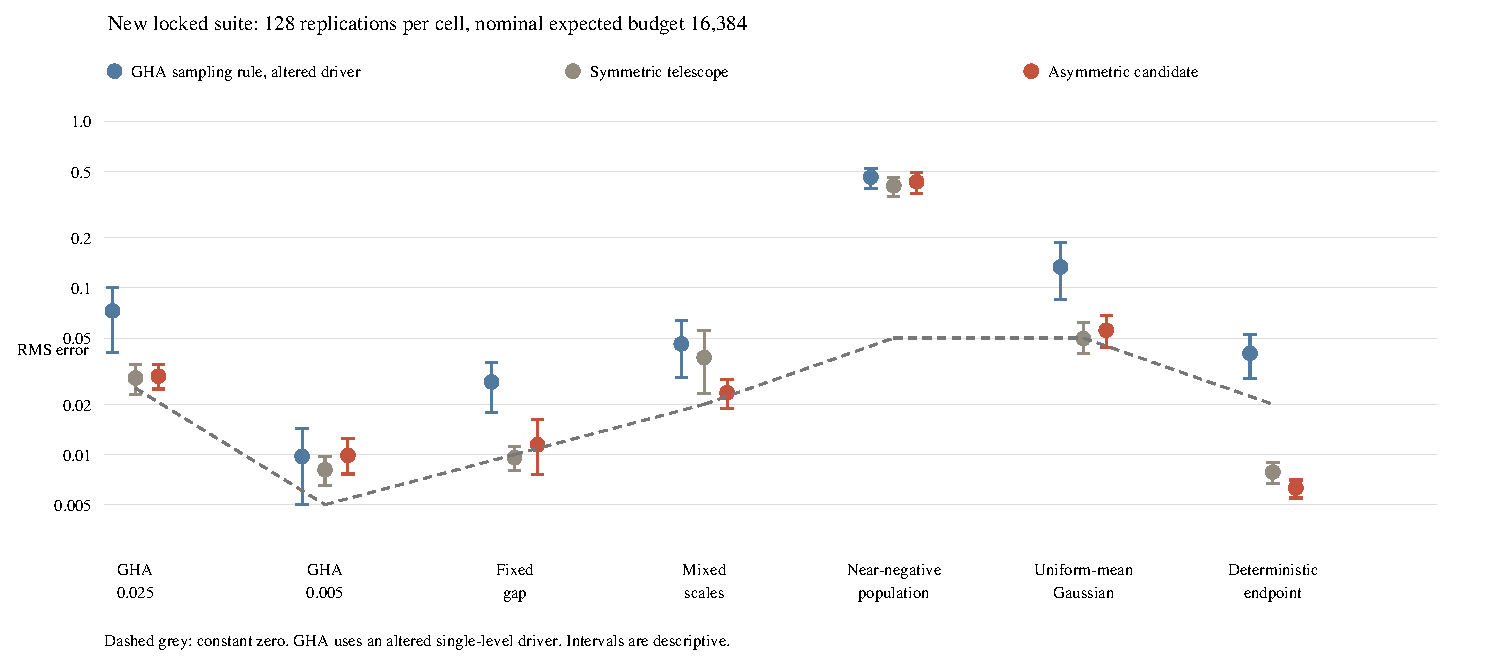
\includegraphics[width=\textwidth]{figures/benchmark.pdf}
 \caption{New held-out numerical evidence, budget 16,384. Error bars are
 descriptive bootstrap intervals. The grey line is the zero-estimator error;
 the GHA curve uses an altered single-level driver. No uniform gain follows.}
\end{figure}

\section{Reproducibility and remaining obligations}
The package contains a claim ledger, dependency graph, source audit, algorithm
contracts, fixed test configuration, raw samples, exact finite diagnostics,
current-source formal audit records, and a failed-approach log. The initial
fourteen numerical/integrity gates passed on a byte snapshot rather than
overwriting historical results. Kernel coverage and any concurrent-source
limitations are specified in \texttt{FORMAL\_COVERAGE.md}; a build verifies
only its audited statements. New statistics are not certified by those builds.

The central unresolved obligation is a universal $\Psi$ upper theorem or a
rigorous counterexample. Even for the quadratic power law, necessity or
removal of $1+\log L$ is open. Unknown-law adaptation outside specified
envelopes, sharp unknown-rarity penalties, and a formal countable-reservoir
realization with all information bounds are not completed here. This is a
finite research checkpoint, not a promise of background continuation.

\begin{thebibliography}{9}
\bibitem{lv} J. C. H. Lee and P. Valiant.
Uncertainty about Uncertainty: Optimal Adaptive Algorithms for Estimating
Mixtures of Unknown Coins. arXiv:1904.09228v3, 2021, Section 7,
Lemmas 17--18 and Corollary 19.
\url{https://arxiv.org/html/1904.09228v3}.
\bibitem{gha} M. B. Giles and A.-L. Haji-Ali.
Multilevel nested simulation for efficient risk estimation.
arXiv:1802.05016v2, 2019, Assumptions 2.1 and 2.4, Theorem 2.7, Algorithm 1.
\url{https://arxiv.org/pdf/1802.05016v2}.
\bibitem{vihola} M. Vihola. Unbiased estimators and multilevel Monte Carlo.
arXiv:1512.01022v4, 2017, Condition 2 and Theorem 3.
\url{https://arxiv.org/html/1512.01022v4}.
\bibitem{blum} A. Blum and L. Hu. Active Tolerant Testing.
COLT 2018, Appendix G.
\url{https://home.ttic.edu/~avrim/Papers/TolerantTesting.pdf}.
\end{thebibliography}
\end{document}
